%!TEX root=../main.tex
\section{Anyagmérleg és moláramok meghatározása}\label{sec:agkompmerl}

A tányéros rektifikáló oszlop paramétereinek beállításához első lépés
a betáplálás áramának és a moltörtek segítségével felállítani a
szükséges anyag- és komponensmérlegeket.
Első lépésként a tömegáramot molárammá számítottuk át a komponensek
móltömege alapján ($M_{víz} = \qty{18.015}{\kg\per\kmol}$, $M_{NMP} =
\qty{99.13}{\kg\per\kmol}$)\autocite{linstromNISTChemistryWebBook1997}:
\begin{equation}
  \begin{split}
    F &= \frac{\dot{m}_F}{M_{atl,F}} \\
    &= \frac{\qty{3900}{\kg\per\hour}}{\qty{74.80}{\kg\per\kmol}} =
    \qty{163.74}{\kmol\per\hour}
  \end{split}
\end{equation}

Az anyag- és komponensmérleget felírva:
\begin{equation}
  \begin{cases}
    F = D + W\\
    F \cdot x_F = D \cdot x_D + W \cdot x_W
  \end{cases}\\
\end{equation}
Behelyettesítve:
\begin{equation}
  \begin{split}
    F \cdot x_F &= D \cdot x_D + (F - D) \cdot x_W\\
    163.74 \cdot 0.30 &= D \cdot 0.85 + (163.74 - D) \cdot 0.02\\
    D &= \qty{55.24}{\kmol\per\hour}\\
    W &= F - D \\
    &= 163.74 - 55.24 = \qty{108.50}{\kmol\per\hour}
  \end{split}
\end{equation}

\section{Tányérszám meghatározása}

A grafikus szerkesztés elvégzése előtt meghatároztuk az elválasztás
sarokpontjait. A betáplált elegy forrásponton (buborékponton) érkezik
az oszlopba, így a betáp hőállapotát jellemző relatív hőigény $q
\approx 1$ (számításainkhoz ---mivel matematikailag hibát okozna a
pontos érték--- 1-hez közeli számot használtunk: \num{0.99999}\dots).
A bináris elegyünk folyadék-gőz egyensúlyi (\emph{vapor-liquid
equilibrium}, VLE) adatait felvázoltuk egy diagramon az illékonyabb
anyag (jelen esetben víz) moltörtjének
függvényében\autocite{pourabadehVLEViscosityModeling2020a}, továbbá
megjelöltük a fontos moltört értékeket (\(x_F\), \(x_D\), \(x_W\)) és
a VLE adatokra az analitikai számítás érdekében hatványfüggvényt
illesztettünk, amelynek alakja az
\ref{fig:yxgraph} ábrán látható, paraméterei pedig:
\begin{equation*}
  \begin{split}
    y \approxeq a\cdot(x-c)^b +d &\qquad R^2\approx 1\\
    a=-0.0222938, \qquad b=-1.45947&, \qquad c=0.0728266, \qquad d=1.01989
  \end{split}
\end{equation*}

\begin{figure}[htbp]
  \centering
  \begin{subfigure}[t][][]{0.45\textwidth}
    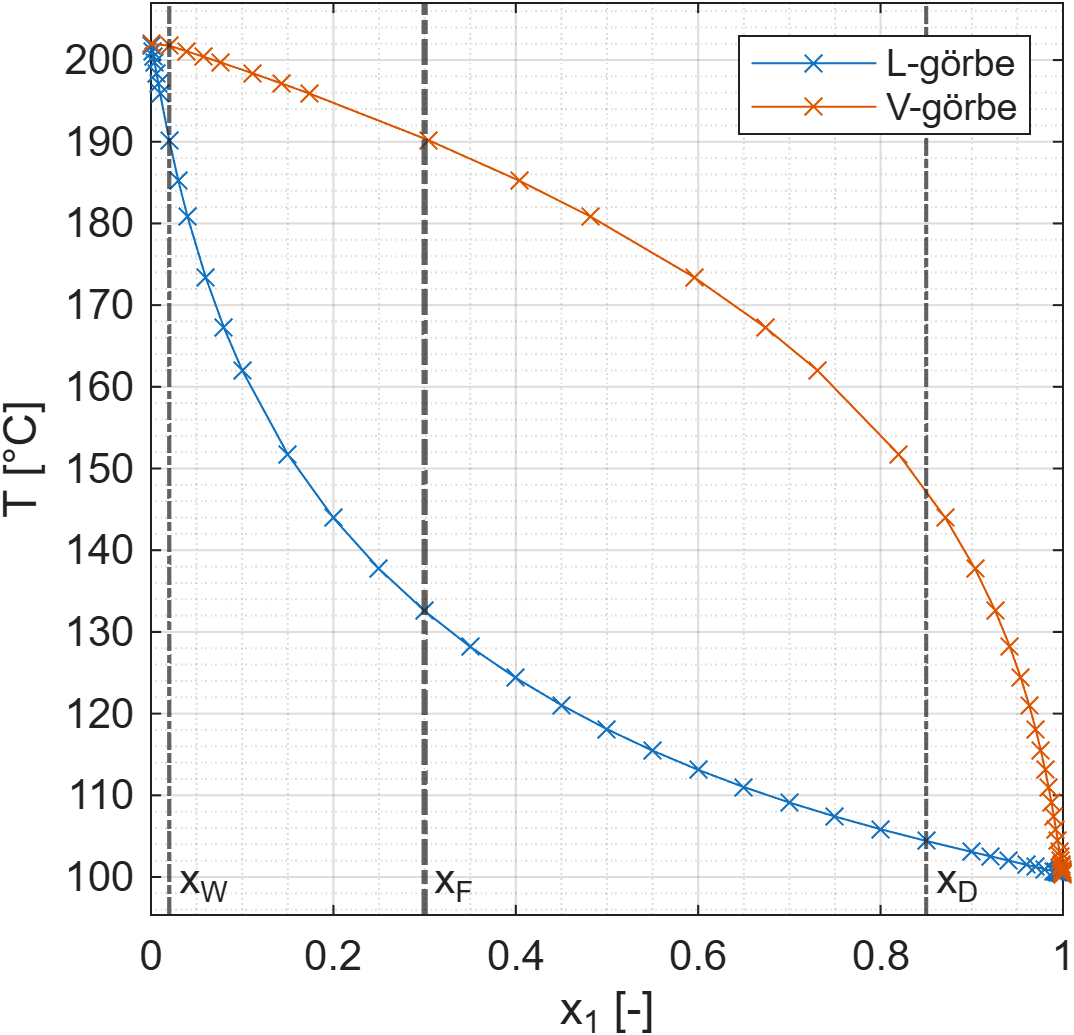
\includegraphics[width=\textwidth]{figures/VLE-WaterNMP-Txy.png}
    \caption{\(T(x;y)\)}\label{fig:Txygraph}
  \end{subfigure}
  \begin{subfigure}[t][][]{0.45\textwidth}
    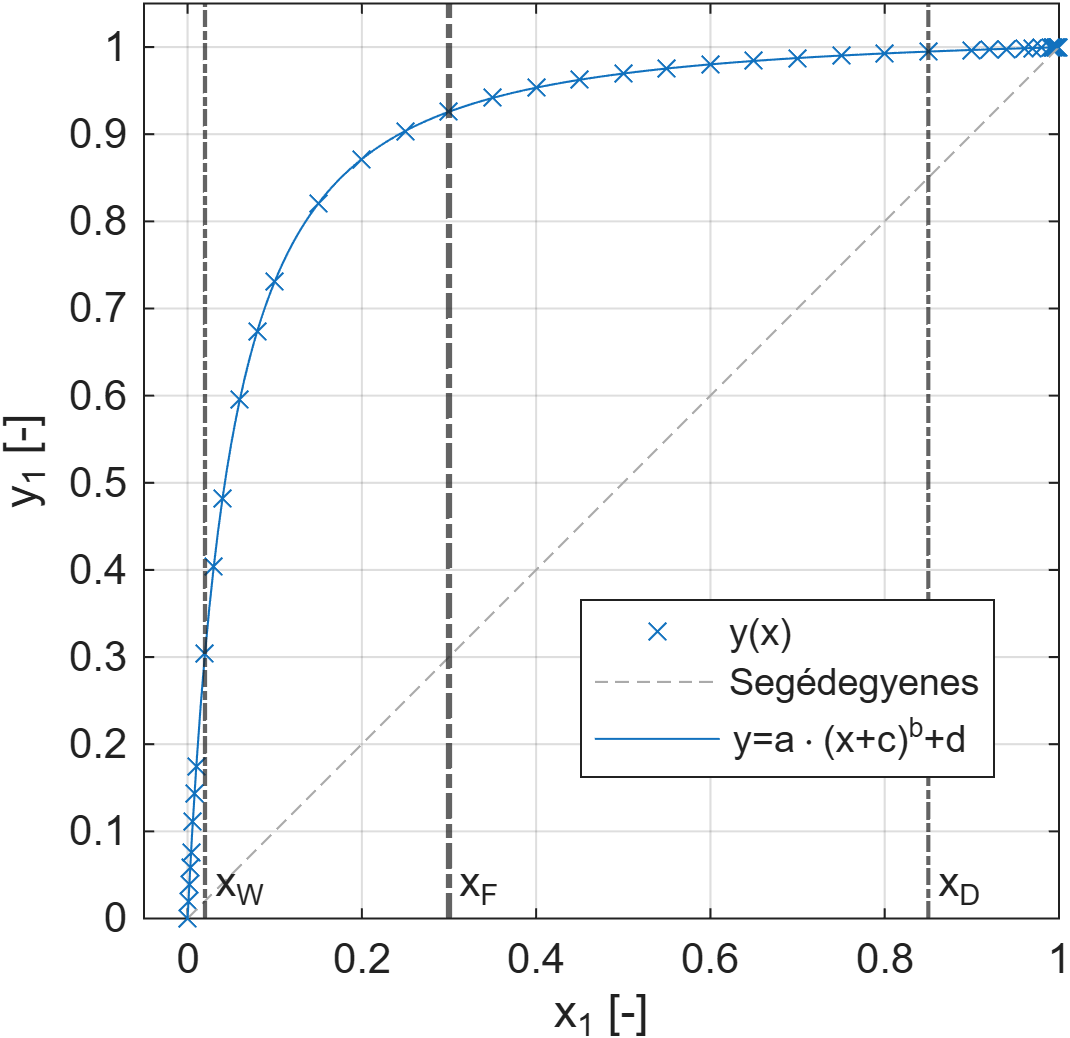
\includegraphics[width=\textwidth]{figures/VLE-WaterNMP-xy.png}
    \caption{\(y(x)\)}\label{fig:yxgraph}
  \end{subfigure}
  \caption{A víz-NMP elegy atmoszférikus folyadék-gőz egyensúlyi diagramjai}
  \label{fig:waterNMPdiags}
\end{figure}

A McCabe-Thiele-féle szerkesztés alternatíva az ideális tányéros
rektifikáló munkavonal-egyenleteinek analitikai megoldására, melyet
akár grafikai programokkal vagy ceruzával, vonalzóval és egy
diagrammal megoldhatunk. A pontosság érdekében mi analitikai
megoldást alkalmaztunk a diagramok fontos pontjainak és értékeinek
megszerkesztése érdekében, amelyet \emph{MatLab}
programmal készítettünk el.

A minimális tányérszám és a minimális refluxarány ``szerkesztéséhez''
meghatároztuk a betáplálás hőállapotából adódó ``q-vonalat'', a dúsító
(felső) és végül a szegényítő (alsó) szakasz
munkavonalainak egyenleteit.

A betáplálási vonal (vagy q-vonal) a dúsító és a szegényítő szakaszok
munkavonalainak metszéspontjait köti össze, miközben áthalad a
betáplálás által meghatározott \((x_F;x_F)\) ponton. A vonal
meredekségét a betáplált elegy termodinamikai állapota (hőállapota),
a $q$ paraméter határozza meg. A vonal általános egyenlete:
\begin{equation}
  y = \frac{q}{q-1}x - \frac{x_F}{q-1}
\end{equation}
ahol \(q=\frac{H_F-h_f}{\lambda_f}\).

A $q$ paraméter fizikai jelentése a betáp egységnyi móláramának
elpárologtatásához szükséges hőmennyiség és a látens párolgáshő
hányadosa. A tervezés egyszerűsítése okából mi ezt forrpontinak,
tehát \(q \approx 1\)-nek vettük.

A felső (dúsító) szakasz munkavonala a gőz- és folyadékáramok mérlegéből
adódik a refluxarány ($R$) függvényében:
\begin{equation}
  y = \frac{R}{R+1}x + \frac{x_D}{R+1}
\end{equation}
Amelyből ha \(x=0\), akkor a tengelymetszet és a refluxarány között
megkapjuk az összefüggést:
\begin{equation}\label{eqn:refluxarany1}
  y = \frac{x_D}{R+1}
  \implies R = \frac{x_D}{y}-1
\end{equation}

Mivel a betáplálás telített folyadék állapotú ($q=1$), a q-vonal
függőleges az $x = x_F = 0.3$ helyen. Ekkor minimális refluxot
feltételezve---tehát a q-vonalon az egyensúlyi görbe metszéspontját
felhasználva---a felső munkavonal tengelymetszetéből
(\(\beta_{\mathrm{Fmv}}=0.96713604\)) kiszámíthatjuk a minimális refluxarányt.
\begin{figure}[htbp]
  \centering
  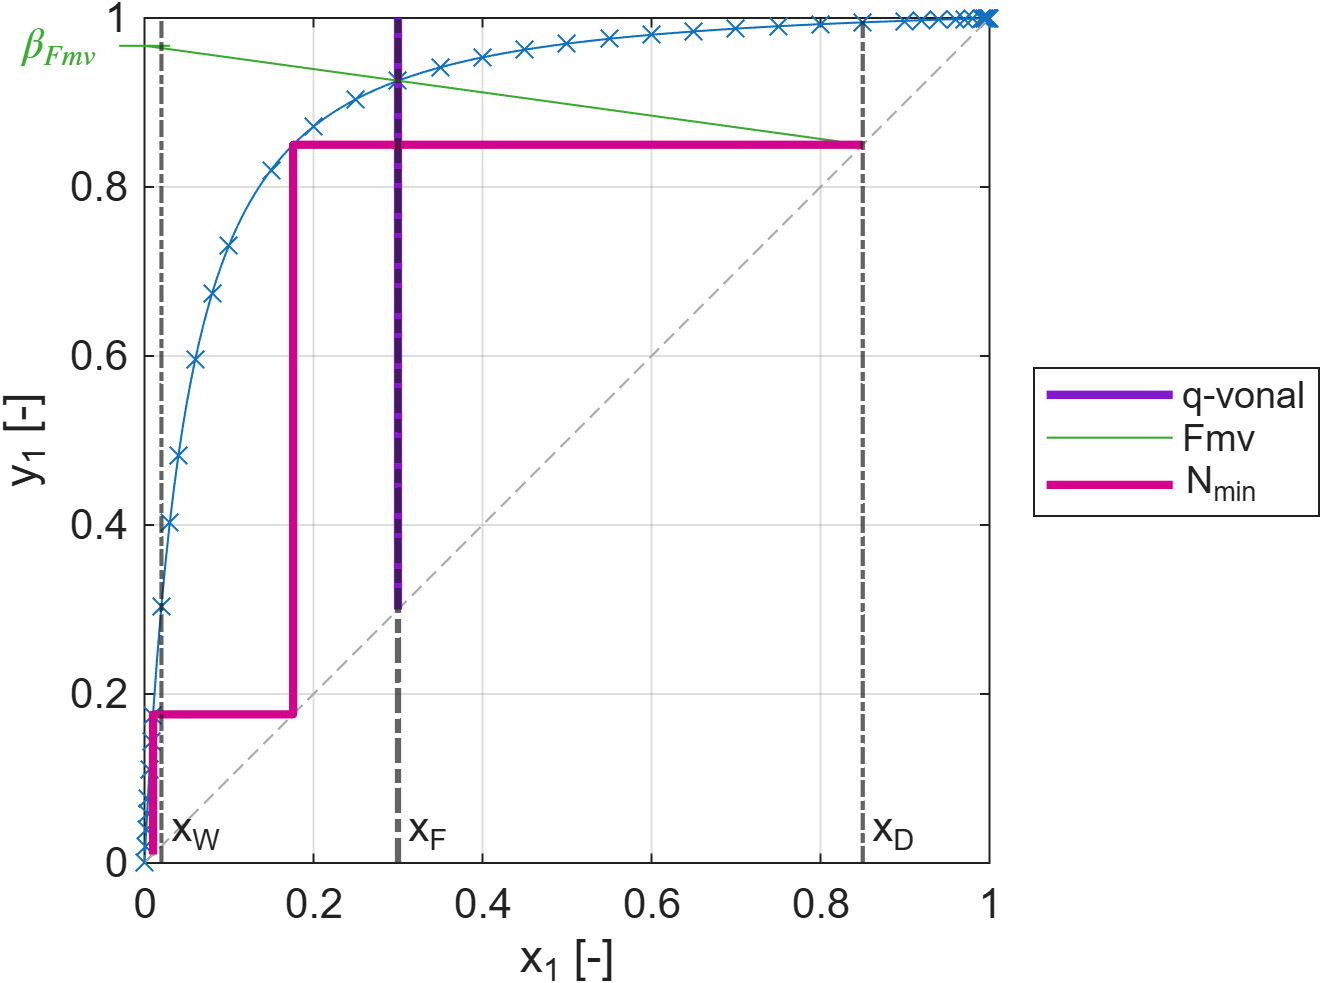
\includegraphics[width=0.5\textwidth]{figures/McGT-Rmin-Nemin.png}
  \caption{Minimális refluxarány és minimális elméleti tányérszám
  számítása lépcsőszerkesztéssel}
  \label{fig:RminandNeminonxy}
\end{figure}

Behelyettesítve az \ref{eqn:refluxarany1} képletbe:
\begin{equation}
  \begin{split}
    \beta_{Fmv} = 0.96713604 &= \frac{0.85}{R_{\mathrm{min}}+1}\\
    R_{\mathrm{min}} &= -0.121
  \end{split}
\end{equation}

A minimális refluxarány számítása fizikailag irreális,
negatív értéket eredményezett ($R_{\mathrm{min}} = -0.121$). Ez abból
adódik, hogy a víz és az NMP között a relatív illékonyság oly
mértékben kedvező, hogy az egyensúlyi görbe alakja alapján a
szétválasztás pusztán elméleti termodinamikai síkon még nulla
folyadék-visszafolyás mellett is megvalósítható lenne.

A diagramon továbbá a minimális elméleti tányérszám
(teljes reflux, azaz végtelen nagy refluxarány mellett) pedig
$N_{\mathrm{min}} = 2$ adódott.

Mivel az oszlop stabil és folyamatos üzeméhez a gyakorlatban
elengedhetetlen a megfelelő folyadék-visszafolyás, egy kellően
alacsony, de stabil üzemet biztosító, kis pozitív refluxarányt
választottunk:
\begin{equation*}
  R = 0,1
\end{equation*}

Az alsó (kiűző vagy szegényítő) szakasz munkavonala a maradék
összetételének megfelelő, az átlón elhelyezkedő $(x_W; x_W)$ pontból
indul, és a dúsító munkavonal, valamint a q-vonal metszéspontján
halad át. Egyenlete a szegényítő szakasz folyadék- ($\bar{L}$) és gőz
moláramainak ($\bar{V}$) ismeretében az alábbi módon írható fel:
\begin{equation}
  y = \frac{\bar{L}}{\bar{V}}x - \frac{W}{\bar{V}}x_W
\end{equation}
Tekintve, hogy a betáplálásunk forrásponti folyadék ($q = 1$), a
folyadékáram a betáplálás moláramával megnő ($\bar{L} = L + q\cdot
F$), míg a gőzáram a két szakasz között változatlan marad ($\bar{V} =
V-(q-1)F$).
\begin{figure}[htbp]
  \centering
  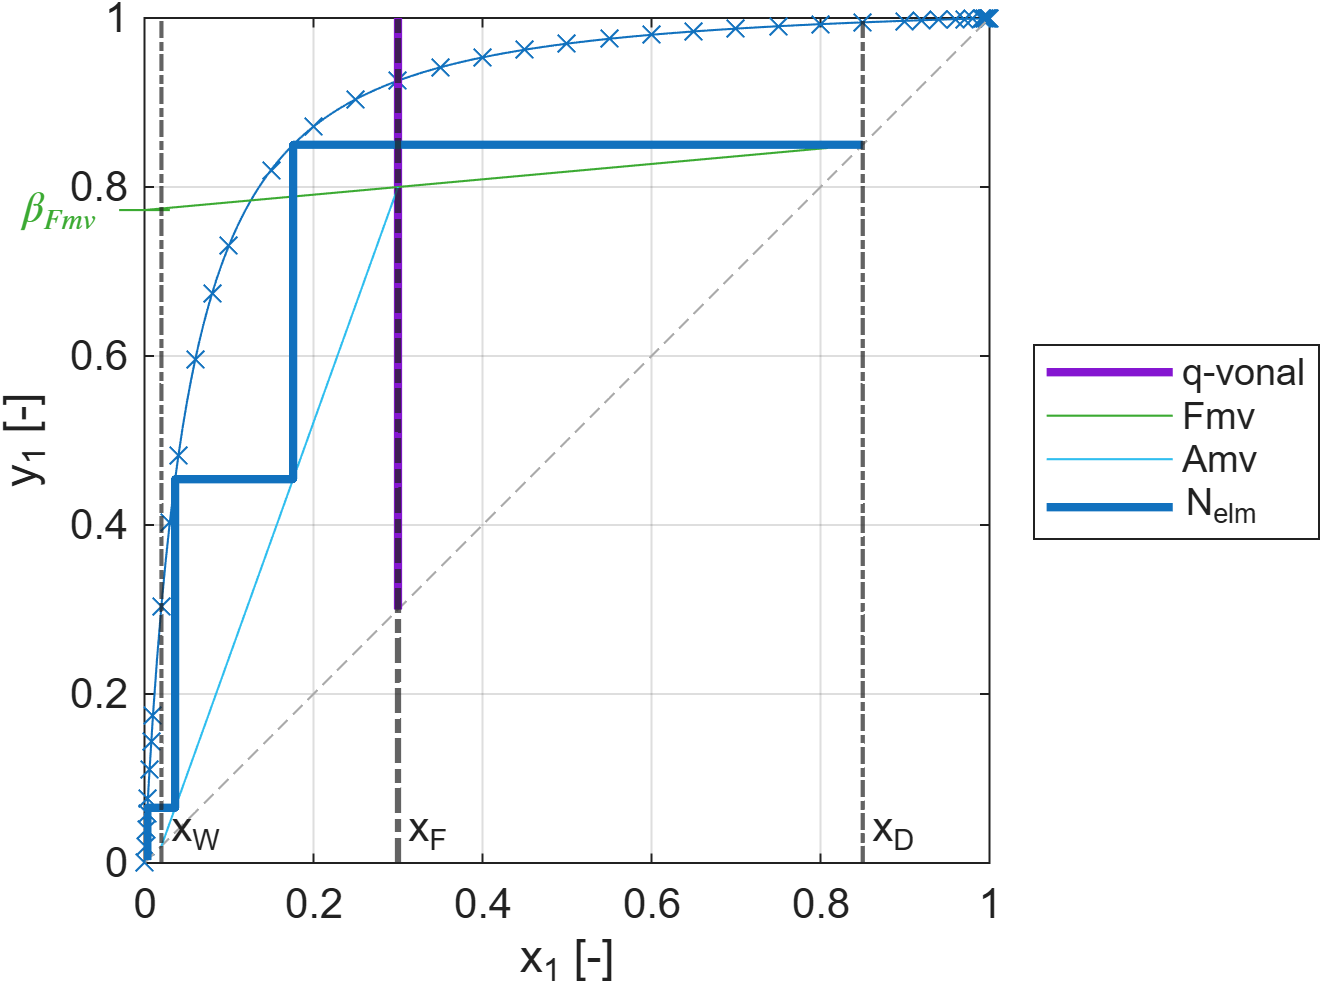
\includegraphics[width=0.5\textwidth]{figures/McGT-Nmin.png}
  \caption{Teljes McGabe-Thiele tányérmeghatározás \(R=0.1, q=1\) esetben}
  \label{fig:mcgabeNelm}
\end{figure}

Ezen $R$ érték mellett, a munkavonalak és az egyensúlyi görbe
ismeretében a McCabe-Thiele szerkesztés lépcsőzését elvégezve a
szükséges elméleti tányérszám:
\begin{equation}
  N_{\mathrm{elm}} = 3
\end{equation}

A valós oszlopmagasság és tányérszám tervezéséhez figyelembe kell
venni a tányérokon fellépő hidrodinamikai és anyagátadási
tökéletlenségeket. Az általunk választott szitatányéros rektifikáló oszlophoz
tartozó átlagos tányérhatásfokot $\eta_T = 0.7$ értéke vettük a
\citetitle{editVegyipariMuveletekII2011} ábrája alapján.
\begin{figure}[htbp]
  \centering
  \includegraphics[width=0.75\textwidth]{figures/Screenshot
  2026-04-15 233636.png}
  \caption{Átlagos tányérhatásfok a terhelési tényező függvényében,
  különböző tányérokra (\protect\citetitle{editVegyipariMuveletekII2011})}
  \label{fig:tanyerhatasfokterhteny}
\end{figure}

A valós tányérszám ($N_{\mathrm{val}}$) meghatározása az elméleti
tányérszám és a hatásfok hányadosaként történik:
\begin{equation}
  N_{\mathrm{val}} = \frac{N_{\mathrm{elm}}}{\eta_T} = \frac{3}{0.7} = 4.28
\end{equation}
A kapott értéket a mérnöki gyakorlatnak megfelelően a következő egész
számra felfelé kerekítettük. Így a beépítendő valós tányérok száma:
\begin{equation*}
  N_{\mathrm{val}} = 5
\end{equation*}

\section{Oszlopátmérő méretezése}

Az oszlop átmérőjét a gőzterhelés és a megengedett gőzsebesség
határozza meg. Az üzemi gőzsebességet a gőzterhelési tényező
($F_{\mathrm{fakt}}$) segítségével számítottuk ki, amelyet az előző
alfejezetben ismertetett diagramról olvastunk le. Az optimális
tányérhatásfokhoz tartozó intervallum két szélsőértékét---ahol a
szitatányér görbéje
elkezd csökkenni---átlagoltuk, ez esetben \numrange{1.0}{2.0}
középértékét használtuk (\(F_{\mathrm{fakt}}=1.5\)).

Továbbá az ideális gáztörvényt felhasználva kiszámítottuk a fejgőz
sűrűségét az atmoszférikus rektifikálóban, ahol a gőz átlagos moláris
tömege a desztillátum moltörtje segítségével számítható:
\begin{equation}
  \overline{M_{D}}=\num{0.85}\cdot \qty{18.02}{\gram\per\mol} +
  (1-\num{0.85})\cdot \qty{99.13}{\gram\per\mol}=\qty{30.18}{\gram\per\mol}
\end{equation}

A gőzsűrűség a fejben ezáltal:
\begin{equation}
  \begin{split}
    \rho_{g,\mathrm{fej}}&=\frac{p\cdot\overline{M_{D}}}{R_{\mathrm{all}}\cdot
    T_{bp}}\\
    &= \frac{\qty{101325}{\pascal}\cdot
    \qty{30.18e-3}{\kilo\gram\per\mol}}{\qty{8.314}{\joule\per\mol\per\kelvin}\cdot\qty{405.65}{\kelvin}}\\
    &= \qty{0.9068}{\kg\per\cubic\metre}
  \end{split}
\end{equation}

Ezekkel együtt a gőz határsebessége:
\begin{equation}
  \begin{split}
    v_{g,\mathrm{fej}} &=
    \frac{F_{\mathrm{fakt}}}{\sqrt{\rho_{g,\mathrm{fej}}}}\\
    &=
    \frac{\qty{1.5}{\sqrt{\pascal}}}{\sqrt{\qty{0.9068}{\kg\per\cubic\metre}}}\\
    &= \qty{1.575}{\metre\per\second}
  \end{split}
\end{equation}

Az átmérő kiszámításához szükséges a fejgőz térfogatárama
($\dot{V}_{V,\mathrm{fej}}$), amelyhez a pára molárama is fontos:
\begin{equation}
  \begin{split}
    V &= (R+1) \cdot D\\
    &= (\num{0.1} + 1) \cdot \num{55.24}\\
    &= \qty{60.76}{\kmol\per\hour}
  \end{split}
\end{equation}
\begin{equation}
  \begin{split}
    \dot{V}_{V,\mathrm{fej}} &= \frac{V\cdot \overline{M_{D}}}{3600
    \cdot \rho_{g,\mathrm{fej}}}\\
    &= \frac{ \cdot 30.18}{3600 \cdot
    2.25}\\
    &= \qty{0.5618}{\cubic\metre\per\second}
  \end{split}
\end{equation}

Az oszlop belső átmérője a kontinuitási egyenletből,
egyszerűsítve\autocite{VegyipariKeszulekekSzerkesztesi1986}:
\begin{equation}
  \begin{split}
    D_b &= \sqrt{\frac{4 \cdot \dot{V}_{V,\mathrm{fej}}}{\pi \cdot
    v_{g,\mathrm{fej}}}}\\
    &= \sqrt{\frac{4 \cdot \qty{0.5618}{\cubic\metre\per\second}}{\pi
    \cdot \qty{1.575}{\metre\per\second}}}\\
    &= \qty{0.6739}{\metre}
  \end{split}
\end{equation}

\section{Az oszlop teljes magasságának meghatározása}

Az oszlop teljes szerkezeti magassága ($H_{\mathrm{tot}}$) három fő
részből tevődik össze: az aktív tányéros szakasz magasságából
($H_{\mathrm{o}}$), a fejmagasságból ($H_{\mathrm{fej}}$), és a
fenékmagasságból ($H_{\mathrm{fenek}}$). Az utóbbi kettőt egybevonva
számítottuk a lentebbieknek megfelelően.

A tányérmagasság meghatározásához a gőz határsebességére és a
gőz-folyadék sűrűségarányra van szükségünk. Mivel a határsebességet
és a gőzsűrűséget már kiszámoltuk, a fejtermék folyadékállapotának
sűsűségét kellett becsülnünk, amelyet tömegtört-súlyozott
átlagolással oldottunk meg (a sűrűségeket \(T_{bp,D}\)-hez közel
  néztük ki, és interpoláltunk
\autocites{peterj.linstromWaterH2OInchI}{peterj.linstromNMethyl2pyrrolidoneC5H9NOInChI}).

\begin{equation}
  \begin{split}
    w_D &= \frac{x_D\cdot M_1}{x_D\cdot M_1 + (1-x_D)\cdot M_2}\\
    &= \frac{\num{0.85}\cdot18.02}{\num{0.85}\cdot18.02 +
    (1-\num{0.85})\cdot99.13}\\
    &=\num{0.507}
  \end{split}
\end{equation}

\begin{equation}
  \begin{split}
    \rho_{f,\mathrm{fej}}&= w_D \cdot \rho_{1} + (1-w_D)\cdot
    \rho_{2}\\
    &=\num{0.507}\cdot\qty{955.39}{\kilo\gram\per\cubic\metre}+
    (1-\num{0.507})\cdot\qty{956.99}{\kilo\gram\per\cubic\metre}\\
    &=\qty{956.18}{\kg\per\cubic\metre}
  \end{split}
\end{equation}
Ezekből az irányadó sűrűségarány:
\begin{equation}
  \begin{split}
    \frac{\rho_{g,\mathrm{fej}}}{\rho_{f,\mathrm{fej}}}
    &=\frac{\qty{0.9068}{\kg\per\cubic\metre}}{\qty{956.18}{\kg\per\cubic\metre}}\\
    &=\num{9.48e-4}
  \end{split}
\end{equation}

Amint azt korábban meghatároztuk, az $N_{\mathrm{val}} = 5$ valós
tányér kell az oszlopba, amelyeknek egyenkénti magassága---avagy
tányérok közötti távolság---a
\citetitle*{VegyipariKeszulekekSzerkesztesi1986} alapján, jó közelítéssel:
\begin{figure}[htbp]
  \centering
  \includegraphics[width=0.75\textwidth]{figures/Screenshot
  2026-04-16 010202.png}
  \caption{Tányérmagasság meghatározása
  (\protect\citetitle*{VegyipariKeszulekekSzerkesztesi1986})}
  \label{fig:tanyermagassag}
\end{figure}
\begin{equation}
  h = \qty{0.4}{\metre}
\end{equation}
Így végül az oszlop aktív magassága:
\begin{equation}
  H_{o} = N_{\mathrm{val}} \cdot h = 5 \cdot
  \qty{0,4}{\metre} = \qty{2,0}{\metre}
\end{equation}

A biztonságos üzemvitel és a fázisok szétválása érdekében kiegészítő
tereket kell biztosítani, ezeket mi az oszlop aktív magasságának
felével becsültük, tehát a teljes oszlopmagasság az aktív rész másfélszerese.

A fentiek alapján a rektifikáló oszlop becsült teljes szerkezeti magassága:
\begin{equation}
  \begin{split}
    H_{\mathrm{tot}} &= H_{o}\cdot\num{1.5}\\
    &= \qty{3,0}{\metre}\cdot\num{1.5}\\
    &= \qty{4,5}{\metre}
  \end{split}
\end{equation}

Ez a magasság biztosítja a technológiai kiegészítők (szintmérők,
tisztítónyílások, csatlakozócsonkok) helyigényét is.

\section{Szitatányér szerkezete}

A tányérok szerkezeti sajátosságaihoz először az oszlop fejgőzének
tulajdonságai mellett az oszlop kigőzölő (alsó) részének is ki
kellett számítanuk a gőz sűrűségét. Ehhez szükségünk volt a
szitatányérok átlagos nyomásesésére, amelyet kezdeti becslésként a
forrásban megadott intervallum számtani közepén vettünk.
\begin{equation}
  \Delta p_T = \frac{300+500}{2}=\qty{400}{\pascal}
\end{equation}

A nyomás az oszlop fenékrészében így a fejbeni atmoszférikus nyomás
és a tányéronkénti nyomásesés szummája:
\begin{equation}
  \begin{split}
    p_{\mathrm{fenek}}&=p_{\mathrm{fej}}+N_{\mathrm{val}}\cdot\Delta
    p_{\mathrm{fenek}}\\
    &=\qty{101325}{\pascal}+\num{5}\cdot\qty{400}{\pascal}\\
    &=\qty{103325}{\pascal}
  \end{split}
\end{equation}

A nyomás alapján az alsó oszloprész gőzsűrűsége:
\begin{equation}
  \begin{split}
    \rho_{g,\mathrm{fenek}}&=\frac{p_{\mathrm{fenek}}\cdot
    \overline{M_{W}}}{R_{\mathrm{all}}\cdot T_{bp,W}}\\
    &= \frac{\qty{103325}{\pascal}\cdot
    \qty{97.51e-3}{\kilo\gram\per\mol}}{\qty{8.314}{\joule\per\mol\per\kelvin}\cdot\qty{463.15}{\kelvin}}\\
    &= \qty{2.6165}{\kg\per\cubic\metre}
  \end{split}
\end{equation}

A szitatányér áthaladó nyílásait a
\citetitle*{VegyipariKeszulekekSzerkesztesi1986} szabályai szerint becsültük.
A tányéron lévő lyukak átmérőjét
\(d_{\mathrm{lyuk}}=\qty{0.005}{\metre}=\qty{5}{\mm}\)-nek vettük,
amihez a megfelelő homogén eloszlás és integritás érdekében a
lyuktávolságot az átmérő háromszorosának
vettük\autocite{VegyipariKeszulekekSzerkesztesi1986}.
\begin{equation}
  \begin{split}
    p_{\mathrm{lyuk}}&=3\cdot d_{\mathrm{lyuk}}\\
    &=\qty{0.015}{\metre}
  \end{split}
\end{equation}

Ezek alapján a tányéroknak szükséges felület a következő képlettel
számítható\autocite{VegyipariKeszulekekSzerkesztesi1986}:
\begin{equation}
  \begin{split}
    A_{\mathrm{szuks}}&=\frac{\dot{V}_{V,\mathrm{fej}}\cdot\sqrt{\frac{\rho_{g,\mathrm{fej}}+\rho_{g,\mathrm{fenek}}}{2}}}{10}\\
    &=\frac{\qty{0.5618}{\cubic\metre\per\second}\cdot
    \sqrt{\frac{\qty{0.9068}{\kg\per\cubic\metre}+\qty{2.6165}{\kg\per\cubic\metre}}{2}}}{\qty{10}{\m\sqrt{\kg\per\metre\cubed}\per\s}}\\
    &=\qty{0.07456}{\metre\squared}
  \end{split}
\end{equation}

Továbbá egy lyuk felülete, ebből a lyukak összessége és egy tányérra
jutó lyukak száma:
\begin{equation}
  \begin{split}
    A_{\mathrm{lyuk}}&=d_{\mathrm{lyuk}}^2\cdot\pi /4\\
    &=(\qty{0.005}{\metre})^2\cdot\pi /4\\
    &=\qty{1.9635e-5}{\metre\squared}
  \end{split}
\end{equation}
\begin{equation}
  \begin{split}
    N_{\mathrm{lyuk}}=\frac{A_{\mathrm{szuks}}}{A_{\mathrm{lyuk}}}\\
    &=\frac{\qty{0.07456}{\metre\squared}}{\qty{1.9635e-5}{\metre\squared}}\\
    &=\num{3797.42}
  \end{split}
\end{equation}
\begin{equation}
  \begin{split}
    N_{\mathrm{lyuk,T}}=\frac{N_{\mathrm{lyuk}}}{N_{\mathrm{val}}}\\
    &=\frac{\num{3797.42}}{\num{5}}\\
    &=\num{759.484} \approx 760
  \end{split}
\end{equation}

\section{Hőmérleg és energiaigény}

A rektifikáló oszlop stacionárius üzemének fenntartásához szükséges
hőáramokat a fázisátalakulásokhoz szükséges energiák alapján határoztuk meg.

\subsection{Kondenzátor hőterhelése}
A fejtermék teljes kondenzálásához és a reflux biztosításához
elvonandó hőáramot ($Q_{kond}$) a gőzáram molárama és a desztillátum
összetételéhez tartozó átlagos párolgáshő határozza meg:
\begin{equation}
  \begin{split}
    \Delta H_{vap,D} &= x_D \cdot \Delta H_{vap,1} + (1 - x_D) \cdot
    \Delta H_{vap,2}\\
    &= 0,85 \cdot \qty{40,73}{\kilo\joule\per\mole} + 0,15 \cdot
    \qty{51,07}{\kilo\joule\per\mole}\\
    &= \qty{42,28}{\kilo\joule\per\mole}
  \end{split}
\end{equation}
\begin{equation}
  \begin{split}
    \dot{Q}_{kond} &= V \cdot \Delta H_{vap,D}\\
    &= \qty{60.76}{\mole\per\second} \cdot \qty{42.28}{\kilo\joule\per\mole}\\
    &= \qty{713,61}{\kilo\watt}
  \end{split}
\end{equation}

\subsection{Reboiler hőterhelése}
A kifőzőben közlendő hőáramot ($Q_{reb}$) a visszapárologtatott
gőzáram ($V'$) és az oszlopalji folyadék párolgáshője alapján
számítottuk. A számítás során figyelembe vettük a táblázat szerinti
entalpiakülönbségeket is:
\begin{equation}
  \begin{split}
    \Delta H_{vap,W} &= x_W \cdot \Delta H_{vap,1} + (1 - x_W) \cdot
    \Delta H_{vap,2}\\
    &= 0,02 \cdot \qty{40,73}{\kilo\joule\per\mole} + 0,98 \cdot
    \qty{51,07}{\kilo\joule\per\mole}\\
    &= \qty{50,86}{\kilo\joule\per\mole}
  \end{split}
\end{equation}
\begin{equation}
  \begin{split}
    \dot{Q}_{reb} &= V' \cdot \Delta H_{vap,W}\\
    &= \qty{16,878}{\mole\per\second} \cdot
    \qty{50864}{\joule\per\mole}\\
    &= \qty{858,49}{\kilo\watt}
  \end{split}
\end{equation}

\subsection{Hűtővíz-szükséglet meghatározása}

A kondenzátorban elvonandó hőáramot ($\dot{Q}_{\text{kond}}$) hűtővíz keringtetésével biztosítjuk. A hűtővíz tömegáramának ($\dot{m}_{\text{hviz}}$) kiszámítása a hűtőközeg oldali hőmérleg alapján történik:
\begin{equation}
    \dot{Q}_{\text{kond}} = \dot{m}_{\text{hviz}} \cdot c_{p, 1} \cdot \Delta T_{\text{hviz}}
\end{equation}

A számításhoz alkalmazott adatok:
\begin{itemize}
    \item Víz fajhője: $c_{p, 1} \approx \qty{4180}{\joule\per\kilo\gram\kelvin}$
    \item Megengedett melegedés: $\Delta T_{\text{hviz}} = \qty{15}{\kelvin}$
\end{itemize}

A szükséges hűtővíz tömegárama:
\begin{equation}
    \dot{m}_{\text{hviz}} = \frac{\dot{Q}_{\text{kond}}}{c_{p, 1} \cdot \Delta T_{\text{hviz}}} = \frac{\num{713,6} \times 10^3}{\num{4180} \cdot 15} \approx \qty{11,38}{\kilo\gram\per\second}
\end{equation}
Átszámítva óránkénti mennyiségre:
\begin{equation}
    \dot{m}_{\text{hviz}} \approx \qty{41,0}{\tonne\per\hour}
\end{equation}

\subsection{Fűtőgőz-szükséglet meghatározása}

A forraló hőigényét ($\dot{Q}_{\text{reb}}$) telített vízgőz kondenzációjával biztosítjuk. Mivel a fenéktermék buborékpontja a számítások alapján $T_{\text{bp}, W} \approx \qty{202}{\celsius}$, a fűtőközegnek ennél magasabb hőmérsékletűnek kell lennie. \qty{230}{\celsius} hőmérsékletű ($p \approx \qty{28}{\bar}$) telített gőzt alkalmazva a párolgáshő $r_{\text{gőz}} \approx \qty{1813}{\kilo\joule\per\kilo\gram}$.

A fűtőgőz tömegárama ($\dot{m}_{\text{gőz}}$):
\begin{equation}
    \dot{m}_{\mathrm{fg}} = \frac{\dot{Q}_{\text{reb}}}{r_{\text{gőz}}}
\end{equation}

Behelyettesítve a forraló számított hőteljesítményét ($\dot{Q}_{\text{reb}} = \qty{858,5}{\kilo\watt}$):
\begin{equation}
    \dot{m}_{\mathrm{fg}} = \frac{\qty{858,5}{\kilo\joule\per\second}}{\qty{1813}{\kilo\joule\per\kilo\gram}} \approx \qty{0,474}{\kilo\gram\per\second}
\end{equation}
Óránkénti gőzfelhasználás:
\begin{equation}
    \dot{m}_{\mathrm{fg}} \approx \qty{1706}{\kilo\gram\per\hour}
\end{equation}

\section{Hőcserélő felületek méretezése}

A számított hőáramok ismeretében meghatároztuk a kondenzátor és a
reboiler szükséges hőátadó felületét a hőátviteli alapegyenletek segítségével.

\subsection{A kondenzátor felületszámítása}
A kondenzátor méretezésénél a hűtőközeg (általunk választott üzemi csapvíz) és a kondenzálódó elegy
közötti logaritmikus közepes hőmérséklet-különbséget ($\Delta
T_{\ln}$) alkalmaztuk. A hőátbocsátási tényező ($k_{kond}$)
meghatározása Nusselt gőzkondenzációs elméletén alapuló iterációval történt\autocite{VegyipariKeszulekekSzerkesztesi1986}.
\begin{equation}
  A_{\mathrm{kond}} = \frac{Q_{\mathrm{kond}}}{k_{\mathrm{kond}} \cdot \Delta T_{\ln}}
\end{equation}
\begin{equation}
  A_{\mathrm{kond}} =
  \frac{\qty{713607}{\watt}}{\qty{171,62}{\watt\per\square\metre\kelvin}
  \cdot \qty{159,79}{\kelvin}} = \qty{26,02}{\square\metre}
\end{equation}

\begin{table}[h!]
\centering
\caption{A kondenzátor iterációs számításának összefoglalása}
\begin{tabular}{lcccc|cc}
\toprule
\textbf{Iteráció} & $\theta_i$ [\unit{\kelvin}] & $\alpha_F$ [\unit{\watt\per\square\metre\kelvin}] & $k$ [\unit{\watt\per\square\metre\kelvin}] & $A$ [\unit{\metre\squared}] & $\theta_{i+1}$ [\unit{\kelvin}] & Hiba [\%] \\ \midrule
1. (kezdeti) & 20,00 & 5006,90 & 169,58 & 26,33 & 5,41 & 269,54 \\
\(\vdots\) & \(\hdots\) & \(\hdots\) & \(\hdots\) & \(\hdots\) & \(\hdots\) & \(\hdots\) \\
Végleges & 3,58 & 7698,29 & 171,62 & 26,02 & 3,56 & 0,46 \\ \bottomrule
\end{tabular}
\end{table}

\subsection{A reboiler felületszámítása}
A reboiler esetén nagynyomású telített vízgőzzel történő fűtést
irányoztunk elő. Mivel mindkét oldalon izoterm fázisátalakulás
(kondenzáció és forrás) zajlik, a közepes hőmérséklet-különbség a két
üzemi hőmérséklet differenciája. A hőátbocsátási tényezőre
($k_{\mathrm{reb}}$) a szakirodalmi adatok\autocite{sinnottCoulsonRichardsonsChemical2005} és az \emph{AISI 316L} szerkezeti acél
anyagi ellenállása alapján tettünk becslést.\autocite{VegyipariKeszulekekSzerkesztesi1986}
\begin{equation}
  A_{\mathrm{reb}} = \frac{Q_{\mathrm{reb}}}{k_{\mathrm{reb}} \cdot \Delta T}
\end{equation}
\begin{equation}
  A_{\mathrm{reb}} =
  \frac{\qty{858492}{\watt}}{\qty{750}{\watt\per\square\metre\kelvin}
  \cdot \qty{30}{\kelvin}} = \qty{38,16}{\square\metre}
\end{equation}

A számított felületek alapján a kondenzátorhoz egy $\approx
\qty{26}{\square\metre}$, a reboilerhez pedig egy $\approx
\qty{38}{\square\metre}$ felületű csőköteges hőcserélő alkalmazását
javasoljuk, amely tartalmazza a szükséges biztonsági tartalékokat is.
